\begin{figure}[htbp]
\centering
\begin{tikzpicture}[font=\small,>=stealth]
\begin{scope}[x=1cm,y=1cm]
\draw[->,gray] (-2.35,0)--(2.65,0) node[right] {$\Re z$};
\draw[->,gray] (0,-2.2)--(0,2.25) node[above] {$\Im z$};
\draw[thick] (0,0) circle (2);
\draw[very thick] (1.777778,0) circle (.222222);
\fill (1,1.732051) circle (1.5pt) node[above right] {$z$};
\fill (1.888889,.19245) circle (1.5pt);
\draw[->] (1.10,1.57)--(1.85,.34);
\draw[dotted] (0,0)--(1,1.732051);
\draw (1.95,.20)--(2.65,.75) node[right] {$t(z)$};
\node[below] at (2,0) {$1$};
\node[above left] at (-1.30,1.4) {$|z|=1$};
\node[align=center] at (0,-2.72)
 {$t(z)=\dfrac{8+z}{9}$\\[3pt]
 $\left|t(z)-\dfrac89\right|=\dfrac19$};
\end{scope}
\begin{scope}[shift={(8,0)}]
\node[align=center] (f) at (0,1.5) {Representación de fase\\[3pt] $r\longmapsto r$};
\node[align=center] (m) at (0,0) {Transporte de memoria\\[3pt] $(r,n)\longmapsto(r,n+1)$};
\draw[->,thick] (f)--(m);
\node[draw,rounded corners,inner sep=8pt,align=center] at (0,-1.65)
 {$1-|t(z)|^2=\dfrac8{81}|1-z|^2$\\[5pt]
 Representación y complemento};
\end{scope}
\end{tikzpicture}
\caption{La coordenatización circular de la compresión nonádica. A la izquierda,
el círculo unidad y su imagen de centro \(8/9\) y radio \(1/9\),
dibujados a la misma escala; se muestra la imagen de \(z=e^{i\pi/3}\).
A la derecha, el retorno de fase se acompaña de avance de memoria.
El balance inferior cuantifica la componente complementaria. Esta figura
representa el mapa \(t\), distinto del factor modal \(q=5/9\) de la
coordenatización central.}
\label{fig:compresion-circular}
\end{figure}
